\chapter{Datová analýza}
Cílem této práce je vytvořit datacentrickou aplikaci, jejímž vstupem mají být data nasbírána z~různých archivů po celé České republice. Tématu sběru těchto dat se již v~minulosti věnovali i jiní studenti a~nyní proběhne pokus o jejich sjednocení a~vytvoření ucelené datové sady použitelné pro web, který má tyto archiválie zobrazovat. Pro každou archiválii jsou potřeba její metadata, seznam URL skenů a~obce, ze~kterých data pocházejí. Informace o obcích musí obsahovat podrobnější informace o okresu, kraji a~RÚIAN, aby bylo možné obec jednoznačně identifikovat z~důvodu kolizí názvů obcí. 
\newpara
Pro vypracování datové analýzy byl zvolen programovací jazyk Python, který je vhodný pro datovou analýzu vzhledem k~čitelné syntaxi a~velké škále podpůrných knihoven pro datovou analýzu. Protokol byl vytvořen v~interaktivním prostředí Jupyter notebook, jež kombinuje zobrazení zdrojového kódu a~výstupů v~podobě grafů. Jupyter notebook dále umožňuje výstup exportovat, a~to například ve formátu PDF. Datové sady byly pro snazší práci nahrány do dataframů knihovny Pandas a~grafy byly vizualizovány knihovnou Matplotlib. Dále proběhla interpretace výstupu datové analýzy. Tento výstup je dostupný v~příloze \ref{appendix:data-analysis-output} Výstup datové analýzy.

\section{Datová sada Dominika Popa }
Datová sada matrik od Dominika Popa \cite{Pop} je distribuovaná ve formátu JSON a~obsahuje detailnější informace pro území jednotlivých archiválií. Datová sada musela být před samotnou datovou analýzou upravena, jelikož využívala dynamický klíč názvu obcí, což po normalizaci vytvářelo velmi řídký dataset znemožňující další zpracování.

\section{Datová sada Jakuba Sokolíka}
Datová sada Jakuba Sokolíka \cite{Sokolik} obsahuje data nejen pro matriky, ale i~pro ostatní typy archiválií a~obdobně jako předešlá datová sada je dostupná ve formátu JSON. Celá datová sada byla dodána v~jednom souboru, který kvůli svojí velikosti nebyl dále použitelný, a~proto byl manuálně rozdělen podle jednotlivých archivů. Před samotnou analýzou bylo nutné opravit překlepy v~klíčích ohledně údajů RÚIAN. Datová sada ve všech grafech obsahuje nejvíce záznamů. Toto je zapříčiněno skutečností, že v případě, kdy archiválie obsahovala více obcí, tak se v datové sadě objeví záznam pro každou obec duplicitně. Tedy datová sada nepracuje se seznamem lokalit, ale pouze s jednou lokalitou a v případě, kdy lokalita obsahuje více obcí, tak se záznam zduplikuje.

\section{Datová sada Jana Valuška}
Datová sada \cite{Valusek} je strukturována do jednotlivých JSON souborů podle archivu a~typu archivního materiálu. Obdobně jako datová sada Jakuba Sokolíka obsahuje data pro matriky i ostatní typy archiválií.

\section{Datová sada obsahující URL snímky}
Datová sada s~URL adresami snímků je organizována podle archivů, odkud data pochází. Data jsou ve formátu JSON, a to až na matriky z~Moravského zemského archivu, který jako jediný je ve formátu XML. Pro účely další analýzy byl vytvořen Python skript, který provedl transformaci na ekvivalentní JSON dokument. Formát dat není napříč celou datovou sadou jednotný, takže v~příloze \ref{appendix:data-analysis-output} je uvedena struktura, jež by vznikla při sjednocení souborů napříč datovou sadou. Při kontrole platnosti uvedených URL adres bylo zjištěno, že funkční odkazy jsou pouze pro Archiv hlavního města Prahy, SOA v~Plzni, SOA v~Litoměřicích a~ZA v~Opavě.

\section{Porovnání datových sad}
V této části práce bude zkoumán vztah jednotlivých datových sad a~proběhne mapování napříč datovými sadami.
\newpara
Jak naznačuje graf \ref{fig:datasets-comparison} porovnávající velikosti jednotlivých datových sad, tak zatímco datová sada Dominika Popa, Jana Valuška a~datová sada s~url adresami skenů obsahují přibližně totožný počet záznamů, tak datová sada od Jakuba Sokolíka obsahuje významně více záznamů, což je zapříčiněno tím, že neobsahuje data pouze pro matriky, ale i~pro jiné typy archiválií, a~v případě, že archiválie pokrývá více obcí, tak je zde záznam duplikován.

\begin{figure}[htbp]
\centering
    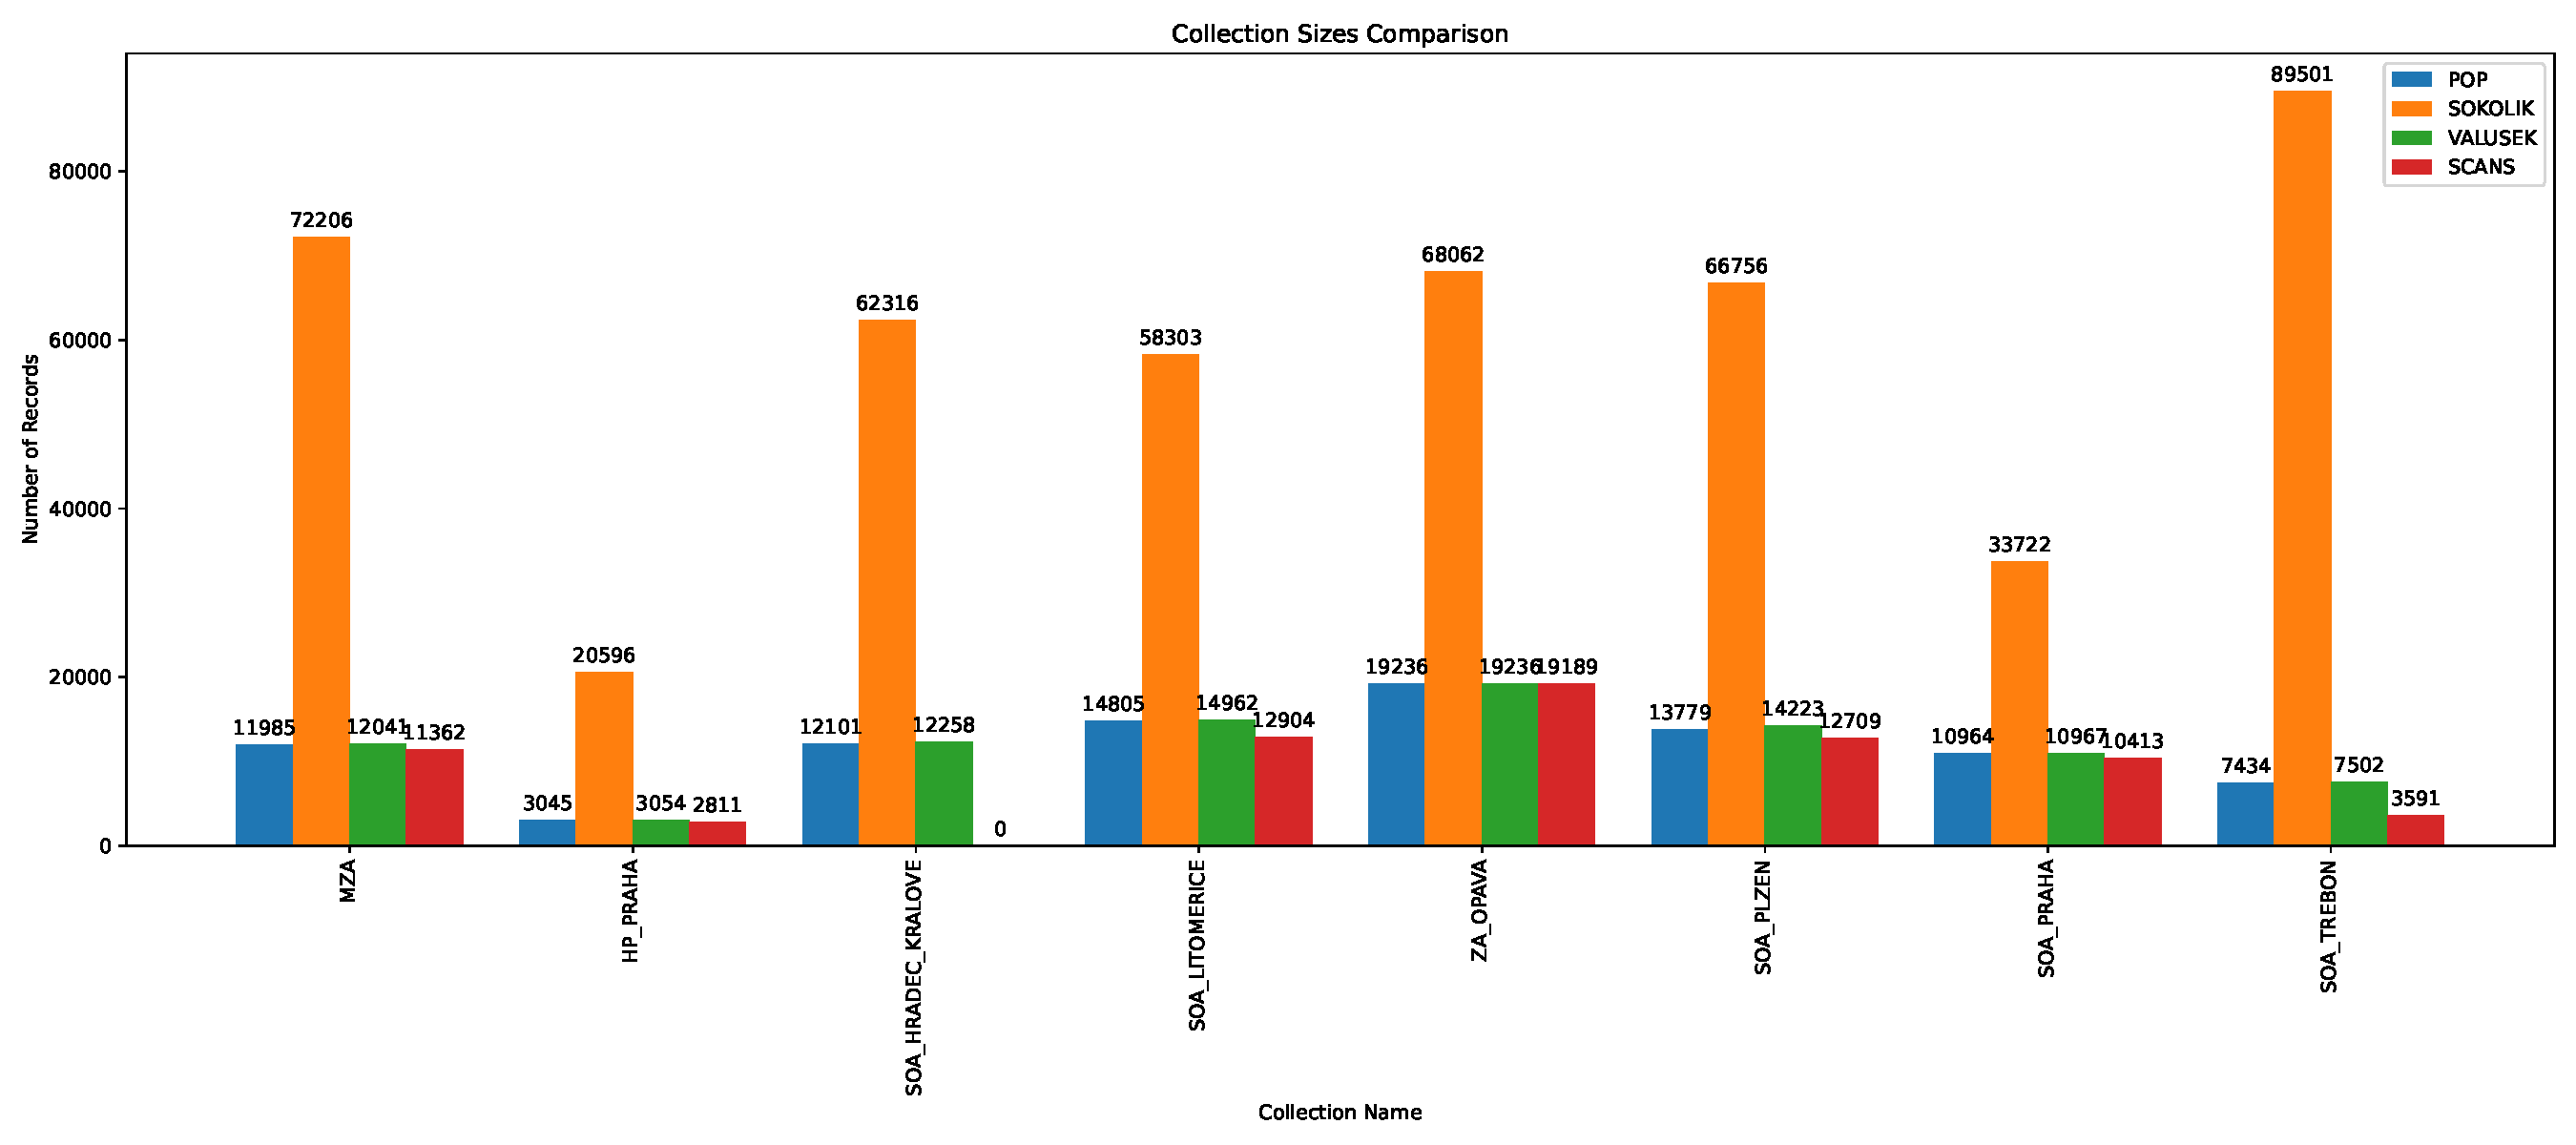
\includegraphics[scale=.3]{obrazky-figures/dataAnalysis/collectionSizesComparison.pdf}
    \caption{Porovnání velikosti jednotlivých datových sad}
    \label{fig:datasets-comparison}
\end{figure}


\subsection{Moravský zemský archiv}
Jak je patrné z~analýzy chybějících hodnot, tak každá datová sada obsahuje vždy jeden identifikátor. V~rámci datové sady Jakuba Sokolíka, Jana Valuška a~sady obsahující skeny se jedná o signaturu, ale v~rámci datové sady Dominika Popa se jedná o inventární číslo. Toto může být zapříčiněno tím, že uživatelské rozhraní Actapublica od MZA používá označení Číslo knihy, což mohlo být jednotlivými autory vyloženo odlišně. Dále proběhlo párování záznamů přes vyplněné identifikátory a~v případě, že se shodují, tak lze předpokládat, že se jedná o totožné záznamy. Napříč datovými sadami neexistuje záznam, který by neměl ani signaturu ani inventární číslo.
Z kontroly duplicit vyplývá, že vyplněné identifikátory v~rámci datových sad jsou jedinečné, a to až na datovou sadu Jakuba Sokolíka, která se potýká s problémem struktury uložení dat. Problém se strukturou dat byl nastíněn v~popisu jeho datové sady, kdy v~případě více vesnic v~rámci jedné archiválie jsou vytvářeny duplicitní záznamy.
Z Vennova diagramu lze vyčíst, že se povedlo namapovat většinu záznamů napříč všemi datovými sadami.
Při kontrole konzistence bylo ověřeno, že data ohledně obcí a~jejich RÚIANy se shodují ve většině případů. Porovnány byly datové sady Dominika Popa a~Jakuba Sokolíka, jelikož jako jediné obsahují RÚIAN identifikátory. Více než 70~\% vesnic se shoduje v~názvu i identifikátoru. V~opačném případě se jednalo převážně o problém, že se nenašel záznam v~obou datových sadách. Neshoda mezi identifikátory nastala u 7~\% záznamů.

\subsection{Archiv hlavního města Praha}

Z analýzy chybějících hodnot vyplynulo, že zde se již autoři shodují v~identifikátorech a~bude tedy stačit porovnat shodu mezi signaturami archiválií.
Z analýzy duplicitních hodnot vyplývá, že signatura je unikátní v~rámci všech datových sad kromě Jakuba Sokolíka, kde duplicity jsou zde opět způsobeny nešťastným strukturováním dat. Při kontrole konzistence bylo zjištěno, že většina záznamů se nachází ve všech datových sadách. Problém nastává u shody obcí v~rámci archiválií, kde se povedlo namapovat pouze 7~\% záznamů. Při detailnějším přezkoumání bylo zjištěno, že Dominik Pop použil detailnější popis oblasti, což způsobuje nekonzistence napříč obcemi. Jako příklad lze uvést, že v rámci datové sady Jakuba Sokolíka je uvedena Praha a~v datové sadě Dominika Popa je uvedeno Staré Město, což je část Prahy a~jedná se o přesnější údaj. I~přes fakt, že obě datové sady mají správné RÚIAN čísla, došlo ke špatnému výsledku mapování, a to kvůli rozdílné úrovni granularity. Všechny záznamy, které se povedlo namapovat, se shodují v~údajích o RÚIANu. Přes 92~\% záznamů se povedlo dohledat i~v~rámci datové sady se skeny, což značí, že tyto výstupy budou použitelné, jelikož pro tento archiv jsou dostupné URL adresy funkční.

\subsection{Státní oblastní archiv v~Hradci Králové}
Pro státní oblastní archiv v~Hradci králové chybí datová sada se skeny a~nejsou tak k~dispozici nascrapované URL jednotlivých snímků. Lze provést pouze porovnání datových sad Jakuba Sokolíka, Jana Valuška a~Dominika Popa, které obsahují informaci o signatuře i~inventárním čísle. Podle analýzy chybějících hodnot bylo odhaleno, že několik záznamů postrádá informaci o~inventárním čísle.
Z analýzy duplicitních hodnot vyplývá, že datové sady Dominika Popa a~Jana Valuška jsou konzistentní a~lze tedy vůči nim porovnávat data z~datové sady Jakuba Sokolíka.
Z~Vennova diagramu lze vyčíst, že dostupné datové sady se shodují u~více jak 9 000 záznamů.
Z výsledků vyplývá, že datová sada Dominika Popa se úplně neshoduje s~obcemi v~druhé datové sadě, každopádně v~případech, kdy daná obec je v~obou datových sadách, tak se ve většině případech RÚIAN identifikátory shodují.

\subsection{Státní oblastní archiv v~Litoměřicích}
Z analýzy chybějících hodnot lze vyčíst, že datové sady Jakuba Sokolíka a~Jana Valuška neposkytují informaci o signatuře ani o inventárním čísle. Pro další analýzu je tedy nelze využít a~budou porovnány pouze signatury ze dvou datových sad.
Duplicity se v~datové sadě Dominika Popa a~další sadě skenů nevyskytují. Mapování datových sad proběhlo úspěšně u většiny záznamů napříč datovými sadami.
Provádět kontrolu konzistence RÚIANů zde není možné, jelikož chybí druhá datová sada, která by tento údaj obsahovala.

\subsection{Zemský archiv v~Opavě}
Z analýzy chybějících hodnot vyplývá, že se zde autoři shodují a~všechny datové sady obsahují údaje o signatuře.
Datová sada Jakuba Sokolíka opět obsahuje duplicity. Zbytek duplicit vyplývá z~chybějících hodnot.
Z Vennova diagramu lze vyčíst, že se datové sady z~velké části shodují. Shoda nastává i mezi názvy obcí a RÚIAN identifikátory.

\subsection{Státní oblastní archiv v~Plzni}
Podle chybějících hodnot zde proběhne mapování záznamů podle signatury, která, kromě již výše zmiňované datové sady Jakuba Sokolíka, nemá duplicity. Celkem se povedlo namapovat přes 9 000 záznamů. Část obcí se povedlo úspěšně namapovat, nicméně několik záznamů vykazovalo chybu.

\subsection{Státní oblastní archiv v~Praze}
Podle chybějících hodnot zde mapování proběhne na základě signatury. Datová sada Dominika Popa byla vyřazena z~důvodu chybějících identifikátorů. Analýza duplicit naznačuje, že se jedná o jedinečné identifikátory. Vennův diagram poukazuje pouze na částečnou shodu mezi třemi datovými sadami a~signifikantní shodu mezi sadou Jana Valuška a~další sadou se skeny. Kontrola konzistence RÚIANů zde opět nemá smysl z~důvodu absence druhé datové sady s~informacemi o obcích.

\subsection{Státní oblastní archiv v~Třeboni}
Všechny datové sady obsahují informaci o signatuře. Analýza duplicit odhalila anomálie, jelikož jsou zde duplicity i~u datových sad, kde doposud žádný problém nebyl. Vennův diagram také naznačuje problém s~mapováním, protože data jsou rozeseta napříč celým diagramem. Mezi datovými sadami byly nalezeny i~různé struktury URL adres, což značí, že možná byla nascrapována různá data napříč sadami.

\subsection{Výsledky datové analýzy}

Většinu datových sad se povedlo namapovat a~vypadá to, že jednotlivé scrapery jsou konzistentní. Standardně by stačilo sloučit datové sady, ale aplikace má podporovat automatické aktualizace, a proto to není možné. V rámci implementovaného systému bude muset být jeden ze scrapovacích systémů integrován.
